
\documentclass[10pt,a4paper]{article}

\usepackage[margin=20mm,top=20mm,bottom=20mm]{geometry}

\usepackage[T1]{fontenc}
\usepackage{lmodern,microtype}
\usepackage{graphicx,booktabs,array,amsmath,amssymb,xcolor}
\usepackage{fancyhdr}
\usepackage{hyperref}
\definecolor{navy}{HTML}{17324C}
\definecolor{muted}{HTML}{53677A}
\hypersetup{colorlinks=true,urlcolor=navy,linkcolor=navy}
\pagestyle{fancy}
\fancyhf{}
\fancyhead[L]{\footnotesize\color{muted} FCC-$\mu e$ Higgs polarization}
\fancyhead[R]{\footnotesize\color{muted} 2 November 2026}
\fancyfoot[C]{\footnotesize\thepage}
\setlength{\headheight}{14pt}
\setlength{\parindent}{0pt}
\setlength{\parskip}{5pt}

\newcommand{\pol}{P_{\mu^+}}

\newcommand{\sqrts}{\sqrt{s}}

\begin{document}
	
{\Huge\bfseries\color{navy} FCC-$\mu e$ Higgs production}\\[5pt]
{\Large Leading-order cross sections and positive-muon polarization}\\[10pt]
{\color{muted}2 November 2026}

\vspace{8pt}\hrule\vspace{12pt}
\textbf{Scope.} Full Standard Model tree-level matrix elements for four final states:
\[
\begin{array}{ll}
\mathrm{CC}: & e^-\mu^+\to\nu_e\bar\nu_\mu H,\quad e^-\mu^+\to\nu_e\bar\nu_\mu HH,\\
\mathrm{NC}: & e^-\mu^+\to e^-\mu^+H,\quad e^-\mu^+\to e^-\mu^+HH.
\end{array}
\]

No imposed generation kinematic cuts; unpolarized $e^-$ beam; $\pol=0,20,40,60,80,100\%$ with $\pol=100\%$ right-helicity antimuons; 
$\sqrts=1$ and 2 TeV, with $(E_e,E_{\mu^+})=(125,2000)$ and $(200,5000)$ GeV, respectively


\vspace{5pt}
\begin{center}
\small
\begin{tabular}{llrrr}\toprule
$\sqrts$ & Channel & $\sigma(0)$ [fb] & $\sigma(80\%)$ [fb] & $\sigma(100\%)$ [fb]\\\midrule
1 TeV & CC $H$ & $210.540\pm0.209$ & $378.570\pm0.243$ & $421.150\pm0.433$ \\
1 TeV & CC $HH$ & $0.074384\pm0.000127$ & $0.133230\pm0.000230$ & $0.148239\pm0.000236$ \\
1 TeV & NC $H$ & $20.835\pm0.025$ & $24.476\pm0.015$ & $25.402\pm0.018$ \\
1 TeV & NC $HH$ & $0.009620\pm0.000015$ & $0.011308\pm0.000017$ & $0.011723\pm0.000018$ \\
2 TeV & CC $H$ & $386.010\pm0.303$ & $695.000\pm0.614$ & $772.690\pm0.517$ \\
2 TeV & CC $HH$ & $0.418510\pm0.000657$ & $0.754495\pm0.001277$ & $0.839521\pm0.001397$ \\
2 TeV & NC $H$ & $38.991\pm0.030$ & $45.829\pm0.055$ & $47.642\pm0.033$ \\
2 TeV & NC $HH$ & $0.054712\pm0.000085$ & $0.064299\pm0.000096$ & $0.066770\pm0.000103$ \\
\bottomrule\end{tabular}
\end{center}




%----------------------------------------------------------
% Figure 1: Absolute cross sections
%----------------------------------------------------------
\begin{figure}[htbp]
\centering
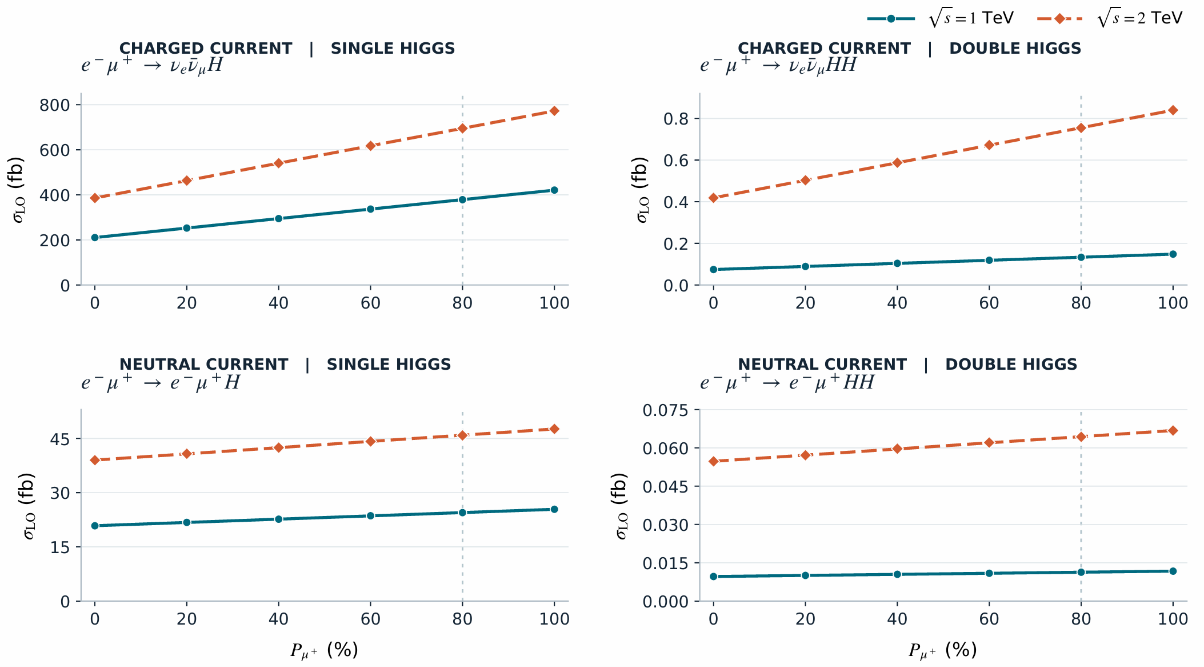
\includegraphics[width=\textwidth]
{1.png}
\caption{
Leading-order Standard Model cross sections for single-
and double-Higgs-boson production in $\mu^+e^-$ collisions
as functions of the longitudinal polarization of the
positive-muon beam, $P_{\mu^+}$.
The four processes considered are
$\mu^+e^-\to\bar{\nu}_{\mu}\nu_e H$,
$\mu^+e^-\to\bar{\nu}_{\mu}\nu_e HH$ (charged current),
and
$\mu^+e^-\to\mu^+e^-H$,
$\mu^+e^-\to\mu^+e^-HH$ (neutral current).
Results are shown for center-of-mass energies of
$\sqrt{s}=1$ and $2$~TeV, with an unpolarized electron
beam and $P_{\mu^+}$ varying from $0\%$ to $100\%$.
The calculations employ the full tree-level Standard
Model matrix elements, without imposing kinematic
phase-space cuts.
Cross sections are expressed in femtobarns (fb).
Error bars represent the Monte Carlo integration
uncertainties.
}
\label{fig: FCCmue_absolute_cross_sections}
\end{figure}


%----------------------------------------------------------
% Figure 2: Polarization enhancement ratios
%----------------------------------------------------------
\begin{figure}[htbp]
\centering
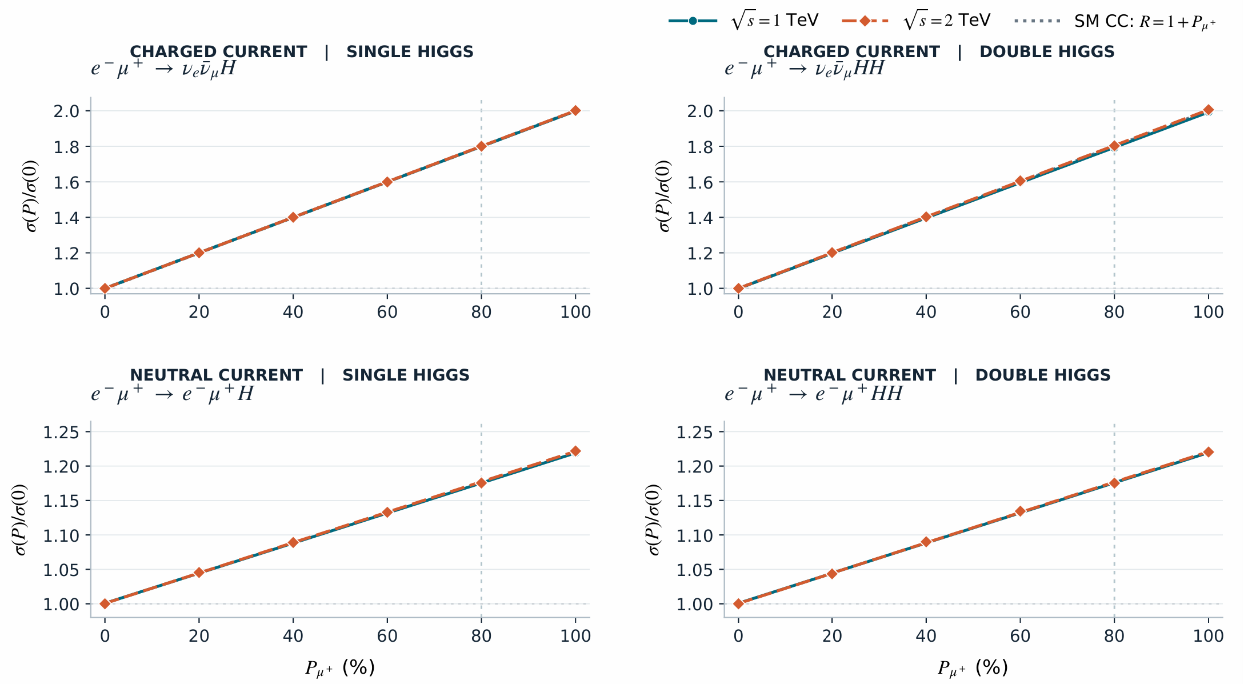
\includegraphics[width=\textwidth]
{2.png}
\caption{
Dependence of the normalized Higgs-production cross
sections on the longitudinal positive-muon beam
polarization in $\mu^+e^-$ collisions.
The polarization enhancement factor is defined as
$R(P_{\mu^+})=\sigma(P_{\mu^+})/\sigma(0)$,
where $\sigma(0)$ denotes the corresponding unpolarized
cross section.
Results are presented for charged-current and
neutral-current single- and double-Higgs production
at $\sqrt{s}=1$ and $2$~TeV.
}
\label{fig: FCCmue_polarization_ratios}
\end{figure}




\newpage
\section*{Inclusive cross sections}

\small

\begin{center}
\setlength{\tabcolsep}{5pt}
\renewcommand{\arraystretch}{1.17}
\begin{tabular}{rrllll}\toprule
$\sqrts$ & $\pol$ & $\sigma(\mathrm{CC}\ H)$ & $\sigma(\mathrm{CC}\ HH)$ & $\sigma(\mathrm{NC}\ H)$ & $\sigma(\mathrm{NC}\ HH)$\\
\mbox{[TeV]} &\mbox{[\%]} & [fb] & [fb] & [fb] & [fb]\\\midrule
1 TeV & 0 & $210.540\pm0.209$ & $0.074384\pm0.000127$ & $20.835\pm0.025$ & $0.009620\pm0.000015$ \\
1 TeV & 20 & $252.710\pm0.158$ & $0.088979\pm0.000149$ & $21.770\pm0.015$ & $0.010045\pm0.000017$ \\
1 TeV & 40 & $294.730\pm0.271$ & $0.104016\pm0.000189$ & $22.660\pm0.014$ & $0.010487\pm0.000016$ \\
1 TeV & 60 & $336.830\pm0.199$ & $0.118825\pm0.000205$ & $23.611\pm0.019$ & $0.010895\pm0.000015$ \\
1 TeV & 80 & $378.570\pm0.243$ & $0.133230\pm0.000230$ & $24.476\pm0.015$ & $0.011308\pm0.000017$ \\
1 TeV & 100 & $421.150\pm0.433$ & $0.148239\pm0.000236$ & $25.402\pm0.018$ & $0.011723\pm0.000018$ \\
2 TeV & 0 & $386.010\pm0.303$ & $0.418510\pm0.000657$ & $38.991\pm0.030$ & $0.054712\pm0.000085$ \\
2 TeV & 20 & $463.490\pm0.399$ & $0.502952\pm0.000846$ & $40.760\pm0.027$ & $0.057089\pm0.000087$ \\
2 TeV & 40 & $540.620\pm0.371$ & $0.587089\pm0.001004$ & $42.460\pm0.045$ & $0.059636\pm0.000086$ \\
2 TeV & 60 & $617.270\pm0.428$ & $0.671917\pm0.001152$ & $44.171\pm0.042$ & $0.062066\pm0.000087$ \\
2 TeV & 80 & $695.000\pm0.614$ & $0.754495\pm0.001277$ & $45.829\pm0.055$ & $0.064299\pm0.000096$ \\
2 TeV & 100 & $772.690\pm0.517$ & $0.839521\pm0.001397$ & $47.642\pm0.033$ & $0.066770\pm0.000103$ \\
\bottomrule\end{tabular}
\end{center}



\section*{Polarization slope and linearity}
We fit the absolute cross section at each energy to
\[
\sigma(\pol)=a+b\,p,\qquad p\equiv\pol/100,\qquad A\equiv b/a,
\]
using weights $1/\delta\sigma_i^2$. Quoted $A$ errors use the fitted covariance matrix and reported integration errors without systematics.


\begin{center}
\small
\begin{tabular}{rllrr}\toprule
$\sqrts$ [TeV] & Channel & $A=b/a$ & $\chi^2/\mathrm{ndof}$ & $p$-value\\\midrule
1 & CC $H$ & $0.9982\pm0.0020$ & $1.77/4$ & $0.779$ \\
1 & CC $HH$ & $0.9934\pm0.0040$ & $2.84/4$ & $0.585$ \\
1 & NC $H$ & $0.2181\pm0.0012$ & $5.08/4$ & $0.279$ \\
1 & NC $HH$ & $0.2186\pm0.0022$ & $1.93/4$ & $0.749$ \\
2 & CC $H$ & $1.0007\pm0.0018$ & $2.38/4$ & $0.667$ \\
2 & CC $HH$ & $1.0053\pm0.0039$ & $0.94/4$ & $0.919$ \\
2 & NC $H$ & $0.2208\pm0.0011$ & $3.40/4$ & $0.493$ \\
2 & NC $HH$ & $0.2204\pm0.0022$ & $3.36/4$ & $0.500$ \\
\bottomrule\end{tabular}
\end{center}

\end{document}



